\chapter{Introducción}
\lettrine{E}{}n un mundo bajo la influencia del Cambio Global es clave conocer la evolución de los ecosistemas para protegerlos mejor. En particular, los ecosistemas acuáticos son fuente de numerosos servicios ambientales, como fuentes de alimentos (incluyendo el agua), medios para el transporte y comercio, servicios turísticos, entre muchos otros. La investigación sobre los impactos del Cambio Global y otras propiedades de los ecosistemas acuáticos se puede realizar mediante el estudio de núcleos sedimentarios, fechados con \PbCero. 
\\
\\
Algunas propiedades químicas y nucleares de \PbCero, las características de los núcleos sedimentarios y el ciclo biogeoquímico de \PbCero\, en sistemas acuáticos se presentan en las Secciones \ref{SubSec-210Pb}, \ref{SubSec-Sedimentos} y \ref{SubSec-Ciclo}.  El fechado de núcleos sedimentarios mediante el modelo de flujo de \PbCero\, constante hacia el sedimento se presenta en la Sección \ref{SubSec-Fechado}. 
\\
\\ 
La medición de la concentración de \PbCero\, en núcleos sedimentarios se realiza mediante espectrometría de rayos gamma, que se describe en la Sección \ref{Secc-IntroEspectrometriaGamma}. La interacción de la radiación con la materia, las características de los detectores de germanio hiper-puro en configuración tipo pozo y la eficiencia del sistema detector - sedimento se muestra en las Secciones \ref{SubSec-Interaccion}, \ref{SubSec-DetecGe}  y \ref{SubSec-Eficiencia}. 
\\
\\ 
La medida correcta de la actividad de \PbCero\, en sedimentos por espectrometría de rayos gamma requiere el conocimiento de la composición química de la muestra, que en este trabajo se determinó mediante espectrometría de fluorescencia de rayos X (Sección \ref{SubSec-XRF-Intro}) y analizador elemental (Sección \ref{SubSec-CN-Intro}). En la Sección \ref{Secc-MonteCarlo} se esbozan ideas generales del método de Monte Carlo utilizado en diversos códigos para calcular las incertidumbres de diversas magnitudes.
\\
\\ 
Finalmente, la hipótesis del presente trabajo y los objetivos, generales y específicos, se encuentran en las Secciones \ref{Sec-Hipotesis} y \ref{Sec-Objetivos}, respectivamente. El objetivo general es analizar la dependencia de la eficiencia, la actividad de \PbCero\, y el fechado de núcleos sedimentarios en función de la composición elemental de cada sección del núcleo. 
\section{Cambio Global y fechado con \PbCero}\label{Sección-1}
El Cambio Global incluye a los cambios observados de manera sistemática a escala planetaria debido a numerosas actividades antropogénicas \cite{CambioGlobal}. Estos incluyen el aumento de la erosión asociada al cambio en el uso del suelo, el deterioro de la calidad de los ecosistemas por contaminantes y el cambio climático causado por la emisión de gases de efecto invernadero \cite{ALowCostLongTerm}. Ante la falta de sistemas de información, observación y monitoreo ambiental a largo plazo, el uso de registros ambientales como anillos de árboles, corales y núcleos sedimentarios es una alternativa para obtener series de tiempo de largo plazo, para lo que es necesario un marco temporal confiable.
\\
\\ 
El marco temporal de los eventos registrados en los núcleos sedimentarios se determina mediante la radiocronología, que permite describir la evolución temporal de los fenómenos registrados a través de algunos radionúclidos, como por ejemplo \PbCero, \Ra\, y \Cs. La elección del radionúclido depende de la escala temporal de interés y del fenómeno a estudiar. 
	\subsection{\PbCero}\label{SubSec-210Pb}
\begin{figure}
 \centering
 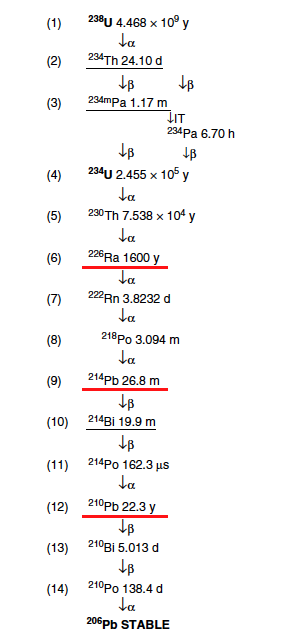
\includegraphics[height=0.8\textheight]{Imagenes/UDacay.png}
 \caption{Serie de desintegración de \UDosTresOcho\, (imagen modificada de \cite{gilmore2008}).}\label{Fig-SerieUranio}
\end{figure}	
\PbCero\, es el radionúclido de principal interés en este trabajo. Se trata de un isótopo radiactivo de Pb, de origen natural, emisor de radiación $\beta^{-}$ (y muy débilmente emisor $\alpha$, con una probabilidad de emisión de 0.0000019 \% \cite{DataDecayEvaluation}) que pertenece a la serie radiactiva de \UDosTresOcho\ (Figura \ref{Fig-SerieUranio}). El 99.25 \% del uranio natural es \UDosTresOcho, que forma parte de la naturaleza de las rocas.
\vspace{0.5cm}
\\
Por otra parte, la actividad $A$ de un radionúclido en una muestra se define como el número de desintegraciones nucleares por unidad de tiempo. La actividad se mide en Becquerelio (Bq) en el Sistema Internacional y es igual al número de desintegraciones nucleares por segundo. La actividad $A$ es proporcional al número de átomos radiactivos $N$ presentes en la muestra en el tiempo $t$ como
\begin{equation}\label{Eq-Desintegracion1}
A = - \dfrac{\text{d}N}{\text{d}t} = \lambda\,N,
\end{equation}
donde la constante de proporcionalidad $\lambda$, conocida como constante de desintegración, depende del núcleo radiactivo y tiene unidades recíprocas de tiempo. El semiperiodo $T_{\frac{1}{2}}$ de un radionúclido es el tiempo en el cual la actividad decrece a la mitad de su valor original. El semiperiodo se relaciona con la constante de desintegración $\lambda$ mediante la ecuación
\begin{equation}
T_{\frac{1}{2}} = \dfrac{\ln(2)}{\lambda}.
\end{equation}
Si $N_0$ y $A_0$ son respectivamente el número de núcleos radiactivos y la actividad en $t=0$, la Ecuación \ref{Eq-Desintegracion1} permite calcular la cantidad de átomos radiactivos $N$ y actividad $A$ en función del tiempo $t$,
\begin{equation}
N(t) = N_0\,\exp(-\lambda\,t), \hspace{2cm} A(t) = A_0\,\exp(-\lambda\,t).
\end{equation}
Para tiempos largos, en series radiactivas como la serie natural de \UDosTresOcho\, (Figura \ref{Fig-SerieUranio}), la actividad del núcleo descendiente $A_{\text{desc}}$ en relación a la actividad del núcleo progenitor $A_{\text{prog}}$ es \cite{gilmore2008}
\begin{equation}
A_{\text{desc}} = \dfrac{T_{\frac{1}{2}, \text{prog}} }{T_{\frac{1}{2}, \text{prog}}  - T_{\frac{1}{2}, \text{desc}}}\, A_{\text{prog}},
\end{equation}
donde $T_{\frac{1}{2}, \text{prog}}$ y $T_{\frac{1}{2}, \text{desc}}$ son los semiperíodos del núcleo progenitor y del núcleo descendiente, respectivamente. Cuando $T_{\frac{1}{2}, \text{prog}} \gg T_{\frac{1}{2}, \text{desc}}$, se produce la igualdad de las actividades, $A_{\text{desc}} = A_{\text{prog}}$, que se conoce como equilibrio secular.
\\
\\
En el caso de un sistema cerrado, los núcleos descendientes de la cadena de \UDosTresOcho\, deberían estar en equilibrio con el progenitor, pues su semiperíodo es muy inferior al de \UDosTresOcho, $T_{\frac{1}{2}}(^{238}\text{U}) = 4.468(5)\times 10^9 \text{ años}$  \cite{DataDecayEvaluation}. Algunos de los descendientes emisores de rayos gamma principales son el $^{234}$Th, $^{234\text{m}}$Pa, \Ra, $^{214}$Pb, $^{214}$Bi y \PbCero\, \cite{gilmore2008}. En sistemas cerrados, \PbCero\, y \Ra se encuentran en equilibrio debido a que estos y los radionúclidos intermedios (por ejemplo \PbCuatro) se encuentran confinados dentro de la matriz ambiental \cite{sanchez2012radiocronologia}.
\\
\\
\PbCero\, tiene un semiperíodo de $T_{\frac{1}{2}}(^{210}\text{Pb}) = 22.23(12)\text{ años}$ \cite{DataDecayEvaluation} y el esquema de desintegración se muestra en la Figura \ref{Fig-Squema210Pb}. El 80.2 \% de los núcleos de \PbCero\, decaen mediante desintegración $\beta^{-}$ al \Bi\, en estado excitado, el cual llega al estado fundamental mediante la emisión de un rayo gamma de 46.539(1) keV. La desintegración $\beta^{-}$ es un proceso de conversión donde un neutrón $n$ se convierte en un protón $p$	, un electrón o partícula $\beta^{-}$ y un antineutrino $\overline{\nu}$ \cite{gilmore2008}. La medida de la actividad de \PbCero\, a través del rayo gamma de 46.54 keV permite fechar núcleos sedimentarios hasta aproximadamente cinco veces el tiempo de vida media, es decir, permite fechar núcleos hasta $\sim$ 100 años de antig\"uedad, lo que incluye la época de mayor crecimiento de población y desarrollo industrial en el planeta, a partir de 1950. 
\begin{figure}[h]
\centering
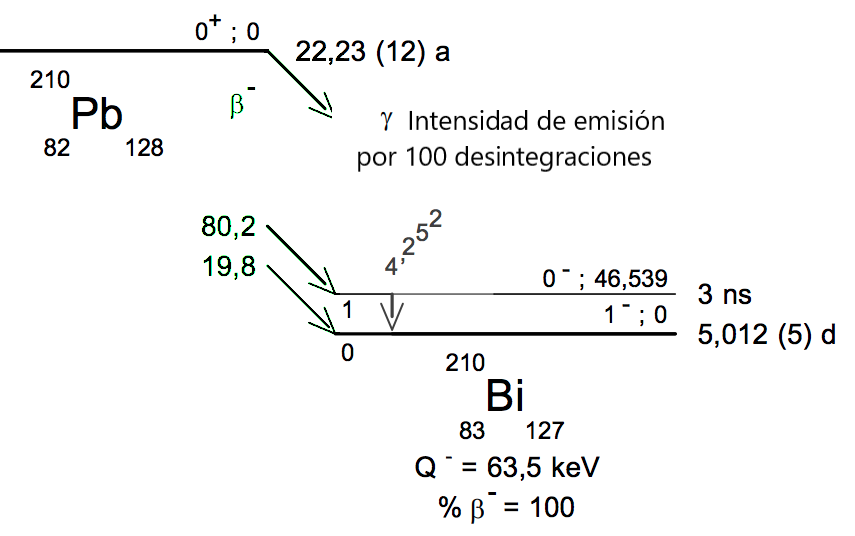
\includegraphics[width=0.5\textwidth]{Imagenes/210Pb-2.png}
\caption{Esquema de desintegración de \PbCero\, \cite{DataDecayEvaluation}.}\label{Fig-Squema210Pb}
\end{figure}
	\subsection{Núcleos sedimentarios}\label{SubSec-Sedimentos}
Para el estudio del Cambio Global se utilizan habitualmente núcleos sedimentarios porque:
\begin{itemize}
\item son concentradores de muchas de las substancias presentes en los sistemas acuáticos (por ejemplo, la mayor parte de los contaminantes),
\item son relativamente fáciles de colectar y analizar, y
\item son integradores de información en el tiempo.
\end{itemize}
Debido a la alta reactividad de Pb con las partículas, el depósito y desintegración de \PbCero\, permite establecer el marco temporal del núcleo sedimentario siempre que se cumpla el principio de superposición, y que los sedimentos no se hayan mezclado después de haber sido depositados.
\\
\\
El muestreo de núcleos sedimentarios se realiza habitualmente en tubos cilíndricos de longitud variable, típicamente del orden de 50 - 100 cm (Figura \ref{Fig-MuestreoNucleoSed}). Los sedimentos pueden ser extrudidos o expuestos longitudinalmente, para ser cortados en secciones de espesor variable (idealmente de 1 cm). La medida de \PbCero\, puede ser realizada directamente mediante espectrometría de rayos gamma (Sección \ref{Secc-IntroEspectrometriaGamma}) o mediante espectrometría de partículas alfa, a través del análisis de su nieto radiactivo \Po, bajo la suposición de equilibrio secular entre ambos radionúclidos (Figura \ref{Fig-SerieUranio}). La espectrometría de partículas alfa requiere un procesamiento radioquímico sencillo, poca cantidad de muestra y permite obtener un recuento rápido de la concentración para obtener una estadística fiable.
\begin{figure}[h]
\centering
  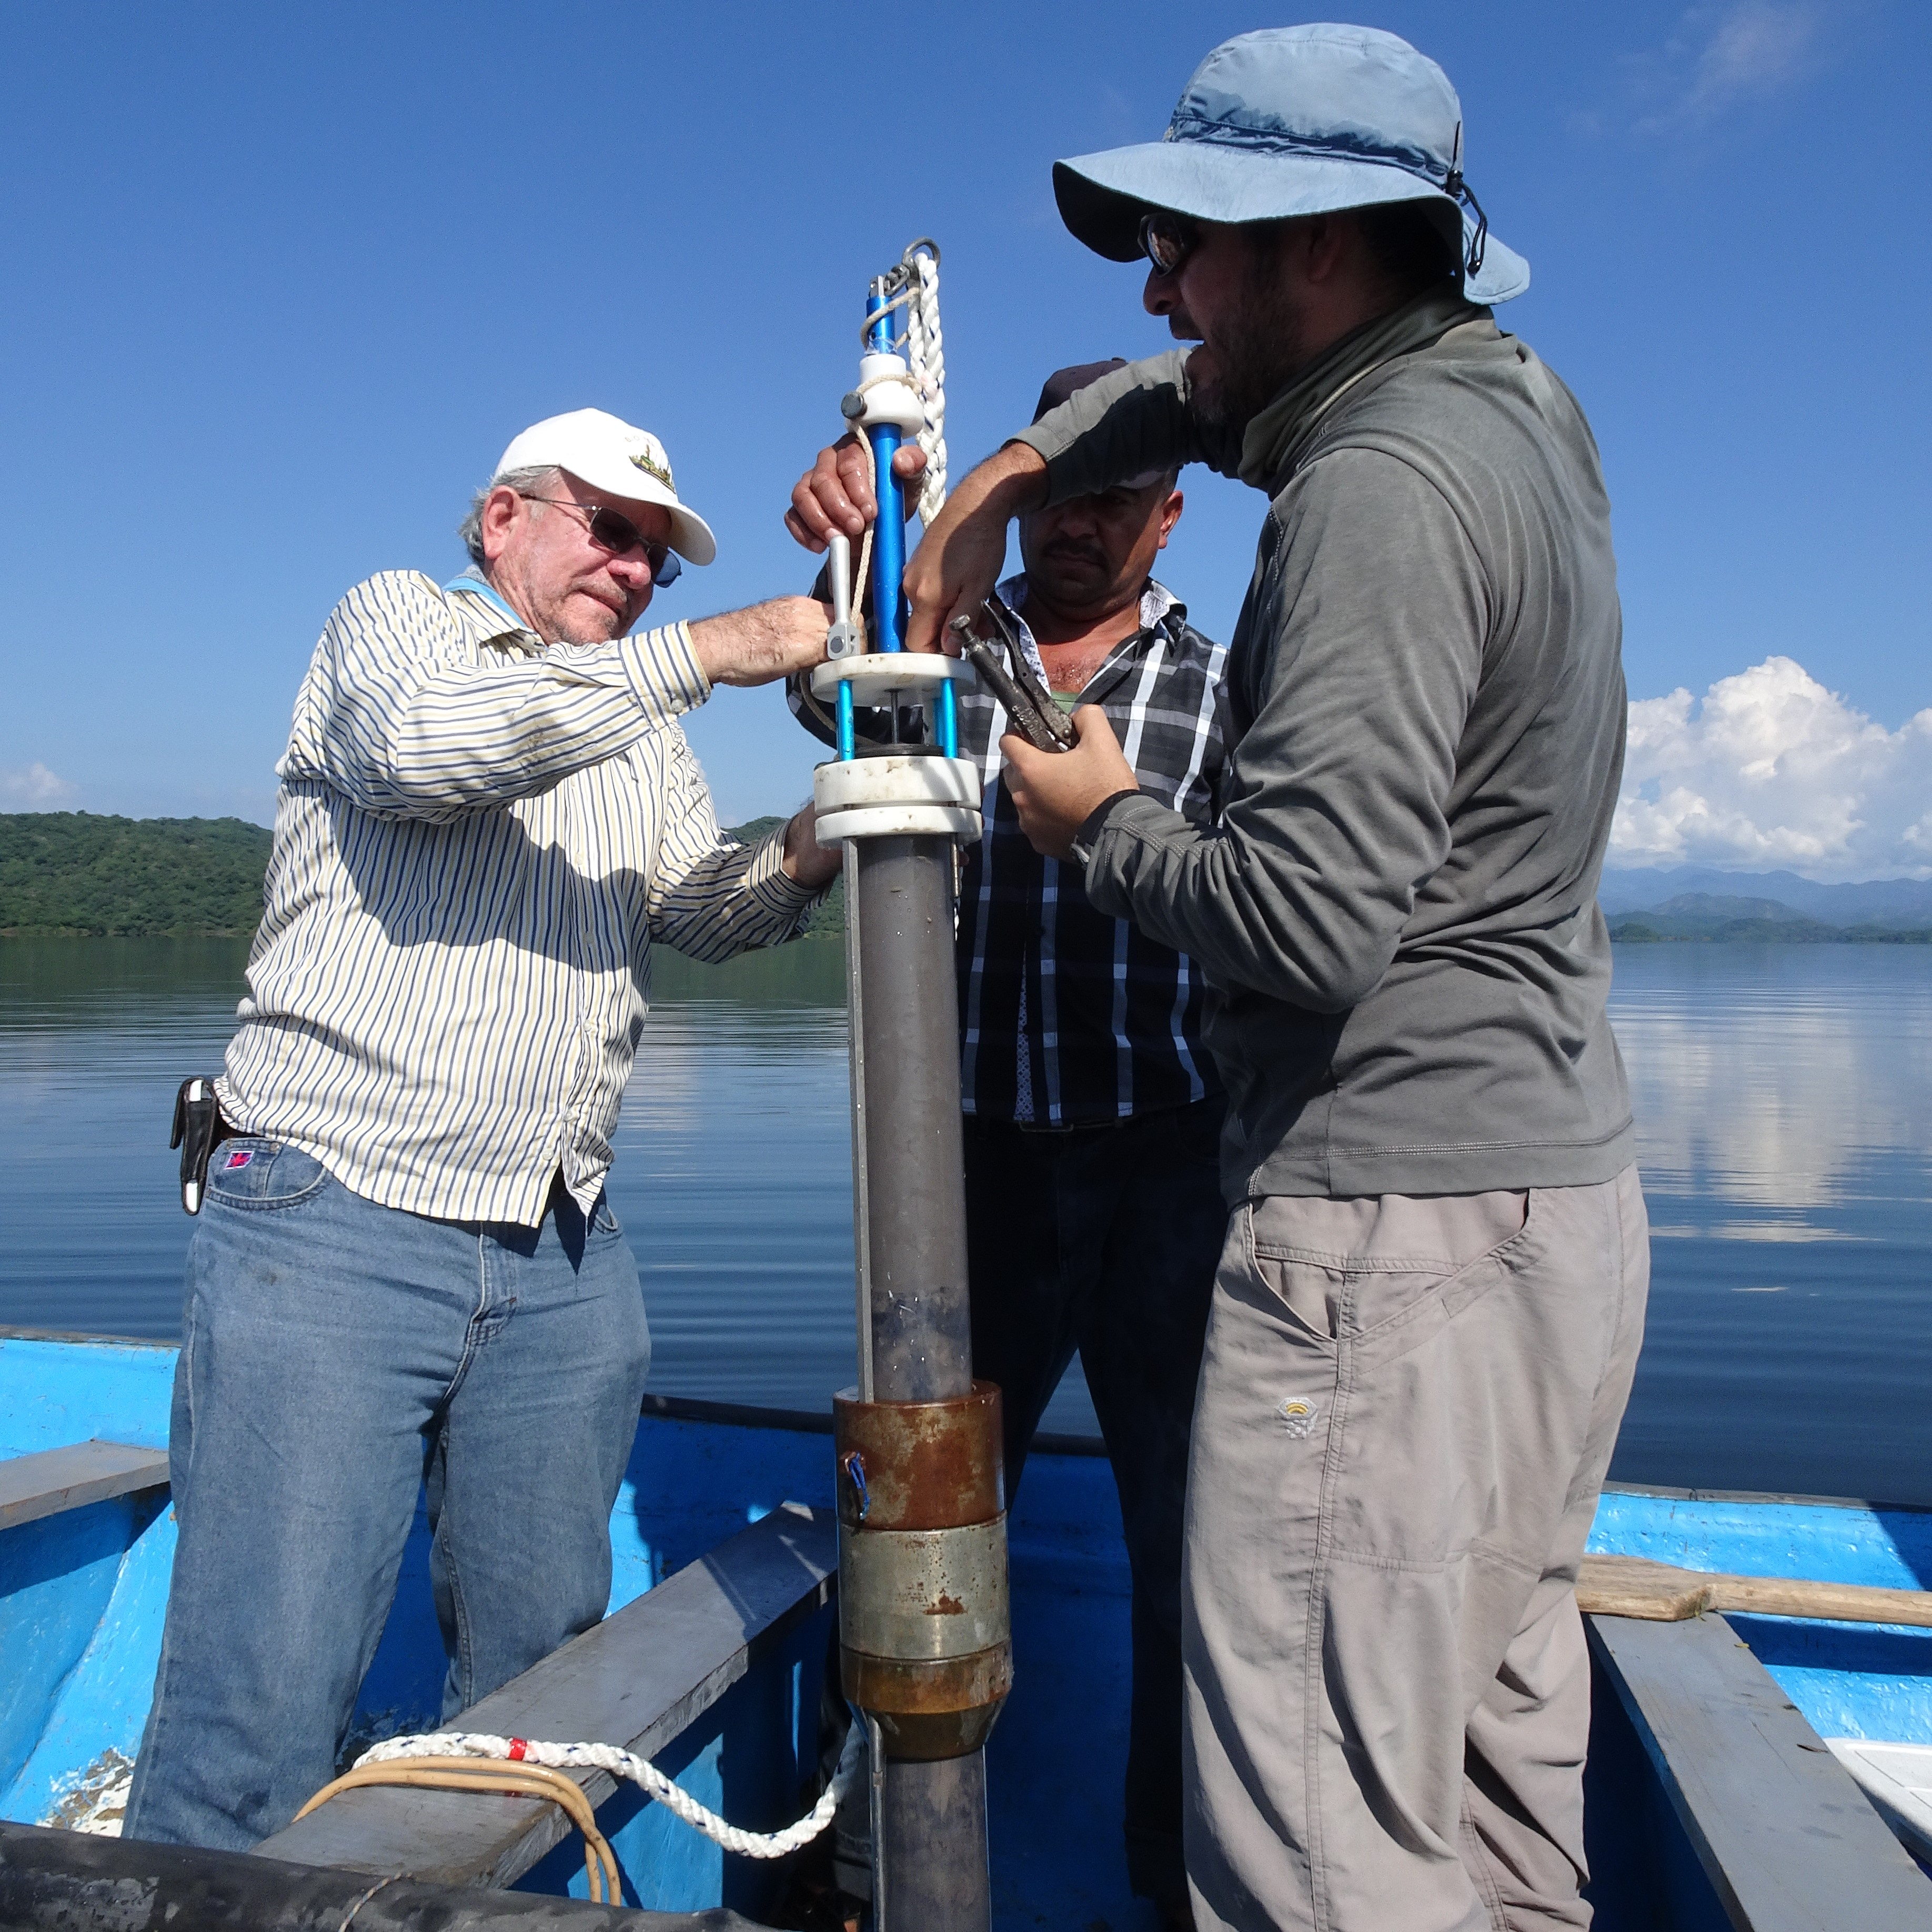
\includegraphics[height = 0.35\textheight]{Imagenes/DSC01875-CUADRADA.JPG}
  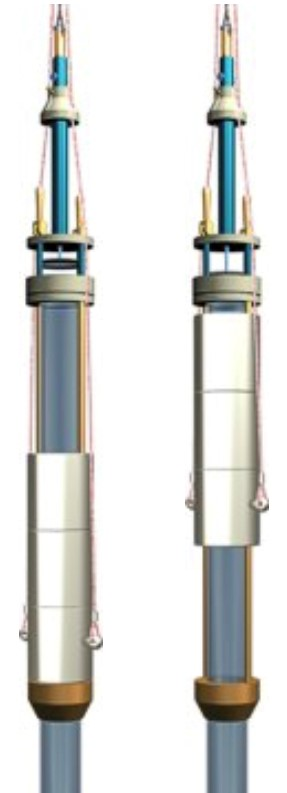
\includegraphics[height = 0.35\textheight]{Imagenes/IMG_2280.jpg}
\caption{Izquierda: muestreo de un núcleo sedimentario en un ambiente lacustre. Derecha: nucleador \cite{Uwitec}.}\label{Fig-MuestreoNucleoSed}
\end{figure}
	\subsection{El ciclo de \PbCero\, en ecosistemas acuáticos}\label{SubSec-Ciclo}
La actividad de \PbCero\, presente en los sedimentos puede tener diversos orígenes (Figura \ref{Fig-Ciclo210Pb}) \cite{KOIDE1972442}:
\begin{itemize}
\item La desintegración de \Rn, núcleo precursor de \PbCero, que es un gas noble y puede escapar de la tierra hacia la atmósfera después de la desintegración del núcleo progenitor \Ra. \Rn\, decae en la atmósfera en una corta serie de núcleos de vida media corta ($\sim$ minutos) hasta \PbCero. Debido a la alta reactividad del Pb con las partículas, el \PbCero\, se une a partículas en suspensión y sedimenta al fondo de los sistemas acuáticos.  
\item \Rn\, puede escapar de la litosfera directamente a los cuerpos de agua y decaer en \PbCero, que también sedimenta al fondo. La suma de este componente y la anterior se denomina \PbCero\, en exceso, \PbCeroEx, que es la base del fechado de sedimentos con \PbCero.
\item \Rn\, que no escapa sino que se desintegra \textit{in situ} y decae en \PbCero, conocido como $^{210}$Pb$_\text{base}$. Para sistemas cerrados por tiempos superiores a 150 años, $^{210}$Pb$_\text{base}$ se encuentra en equilibrio con el radionúclido \Ra\, \cite{SANCHEZCABEZA2012183}, con $T_{\frac{1}{2}}$ (\Ra) = 1600(7) años \cite{DataDecayEvaluation}. 
\end{itemize}
\begin{figure}[h]
 \centering
 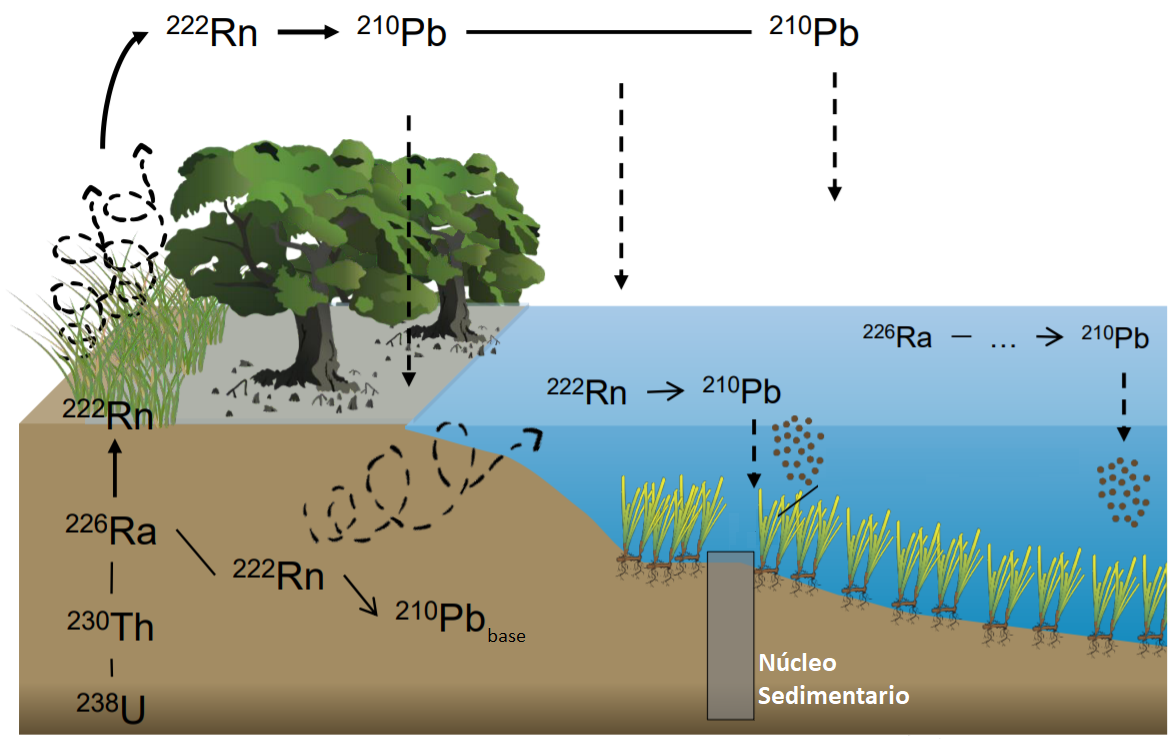
\includegraphics[width=\textwidth]{Imagenes/Ciclo210PbAcuatico.png}
 \caption{Ciclo de \PbCero\, en un sistema costero. Figura tomada de \cite{Foto210Pb}.}\label{Fig-Ciclo210Pb}
\end{figure}
La actividad total medida de \PbCero\, ($^{210}$Pb$_\text{total}$) es la suma de los procesos anteriores:
\begin{equation}\label{Eq-PbTotal}
^{210}\text{Pb}_\text{total} = ^{210}\text{Pb}_\text{base} + ^{210}\text{Pb}_\text{exc}.
\end{equation}
	\subsection{Fechado de núcleos sedimentarios}\label{SubSec-Fechado}
Los modelos de fechado de núcleos sedimentarios son utilizados para \cite{SANCHEZCABEZA2012183}
\begin{itemize}
\item Obtener la edad $t$ de cada sección del núcleo sedimentario en función de la profundidad $z$, es decir, construir un modelo de edad.
\item Calcular tasas de acumulación másica (MAR, en g cm$^{-2}$ año$^{-1}$) y sedimentarias (SAR, en cm año$^{-1}$) en función del tiempo.
\end{itemize}	
Un núcleo sedimentario se puede estudiar como la suma de secciones $i$, Figura \ref{Fig-EsquemaNucleoSed}. Cada sección $i$ presenta ciertas características definidas: masa, densidad, composición elemental, tiempo promedio de formación, actividad de \PbCero, entre otras, y a su vez, cada sección se encuentra en medio de las capas de corte. La nomenclatura de la sección $i$-ésima es un subíndice $_i$ y las capas se denotan mediante paréntesis $(i)$. 
\begin{figure}[h]
 \centering
 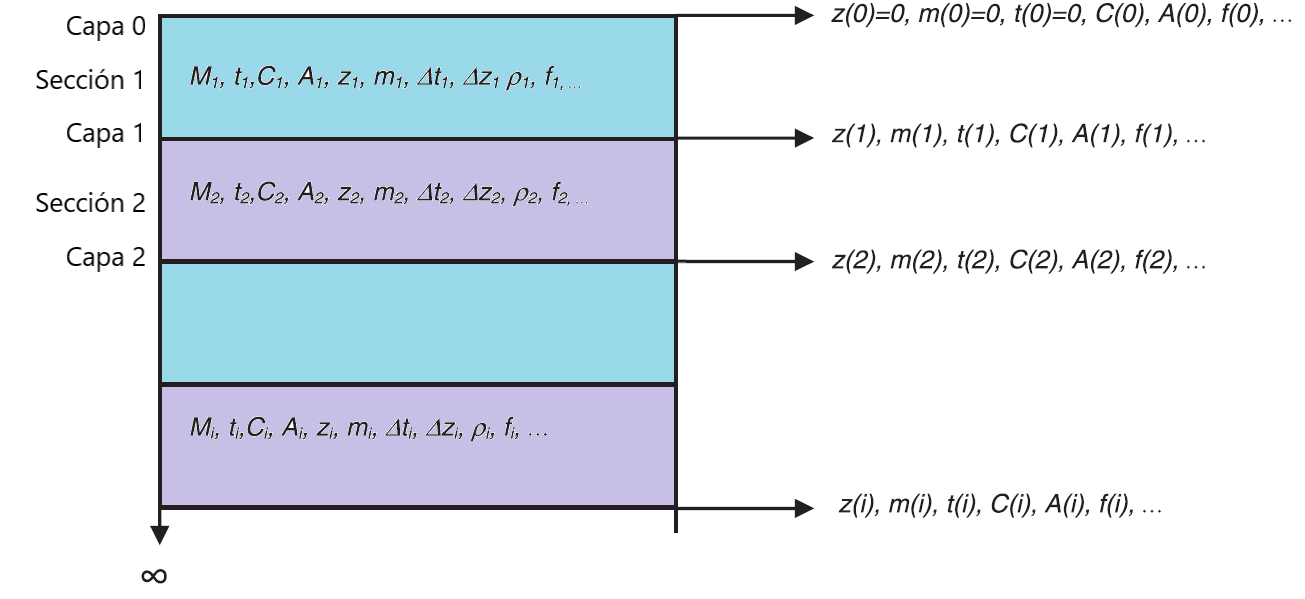
\includegraphics[width=\textwidth]{Imagenes/EsquemaNucleoSed-3.png}
 \caption{Parámetros relacionados con el fechado de un núcleo sedimentario. Imagen modificada de \cite{SANCHEZCABEZA2012183}.}\label{Fig-EsquemaNucleoSed}
\end{figure}	
\\ Algunos parámetros, constantes y definiciones relacionadas con el proceso de fechado son:
\begin{itemize}
\item $T_{\frac{1}{2}}$, $\lambda$: Tiempo de vida media y constante de desintegración del \PbCero, respectivamente. $T_{\frac{1}{2}} = (22.23 \pm 0.12)$ años, $\lambda = (0.03118 \pm 0.00017)$ años$^{-1}$.
\item $S$: Área transversal del núcleo sedimentario. Se calcula utilizando el diámetro interno del núcleo. 
\item $z(i)$: profundidad de la capa $i$-ésima. $z(i=0)=0$ m. 
\item $z_i$: profundidad promedio de la sección $i$-ésima, $z_i = \dfrac{z(i+1)+z(i)}{2}$. 
\item $\bigtriangleup z_i$: ancho de la sección, usualmente próximo a 1 cm. 
\item $\bigtriangleup m_i$: masa seca de la sección $i$-ésima determinada experimentalmente. 
\item $m(i)$: profundidad másica de la capa $i$-ésima. El proceso de fechado debe realizarse en función de la profundidad másica y no en función de la profundidad para tener en cuenta la compactación  del núcleo. $m(i) = \displaystyle \sum_{j=1}^{j=i} \dfrac{\bigtriangleup m_j}{S}$, $m(0) = 0$.
\item $m_i$: profundidad másica promedio de la sección $i$-ésima. 
\item $\rho_i = \dfrac{\bigtriangleup m_i}{S\, \bigtriangleup z_i}$: densidad promedio seca de la sección $i$. 
\item $t(i)$: tiempo transcurrido desde la formación de la capa $i$, $t(0)=0$ años.
\item $\bigtriangleup t_i = t(i) - t(i-1)$: periodo de formación de la sección $i$. 
\item $A_i$: Actividad específica de \PbCeroEx\, de la sección $i$-ésima. 
\item $A_i (t=0)$: Actividad específica de \PbCeroEx\, de la sección $i$-ésima cuando se formó. 
\item $A(i)$: Actividad específica de \PbCeroEx\, de la capa $i$-ésima. 
\item $\bigtriangleup \mathbb{A}_i$: depósito de \PbCeroEx\, en la sección $i$, actividad por unidad de área. $\bigtriangleup \mathbb{A}_i = \dfrac{A_i\,\bigtriangleup m_i}{S}$
\item $s(i)$, $s_i$: tasa de acumulación sedimentaria de la capa $i$ y promedio de la sección $i$, respectivamente. 
\item $r(i)$, $r_i$: tasa de acumulación másica de la capa $i$ y promedio de la sección $i$, respectivamente. 
\item $f(t)$, $f_i$, $f(i)$: flujo a la superficie del sedimento, flujo promedio hacia la superficie del sedimento durante la formación de la sección $i$ y flujo hacia la capa $i$ cuando fue formada, respectivamente. 
\end{itemize}
Cuando la capa $i$-ésima es formada ($t=0$), la concentración de la capa $A(i, t=0)$ es
\begin{equation}\label{Eq-Ci}
A(i, t=0) = \dfrac{f(i)}{r(i)}.
\end{equation}
El modelo de Flujo Constante (CF, por sus siglas en inglés) asume que el flujo de \PbCeroEx\, hacia la superficie del sedimento es constante. $f_i = f(i) = f$. La Ecuación \ref{Eq-Ci} en el modelo de Flujo Constante se puede rescribir como 
\begin{equation}\label{Eq-FC}
f = A(i,t=0)\, r(i).
\end{equation}
La anterior ecuación implica que las concentraciones iniciales $C(i, t=0)$ y la tasa de acumulación másica $r(i)$ de diferentes capas pueden ser diferentes pero deben ser inversamente proporcionales. 
\\ \\ 
El depósito acumulado hasta la capa $i$-ésima $\mathbb{A}(i)$ es 
\begin{equation}
\mathbb{A}(i) = \sum_{j=i+1}^{j\rightarrow \infty} \bigtriangleup \mathbb{A}_j = \int_m^\infty A\, dm =  
\int_m^\infty \dfrac{f}{r}\,\exp(-\lambda\,t)\, dm =  \dfrac{f}{\lambda}\,\exp(-\lambda\,t).
\end{equation}
Para $t=0$, $z=0$ y $m=0$, entonces 
\begin{equation}
f = \lambda\,\mathbb{A}(t=0),
\end{equation}
donde $\mathbb{A}(t=0)$ es el flujo de \PbCeroEx\, en la superficie del sedimento. Entonces el depósito acumulado por debajo de la la capa $i$-ésima es 
\begin{equation}
\mathbb{A}(i) = \mathbb{A}(0)\,\exp(-\lambda\,t).
\end{equation}
De la anterior ecuación se puede calcular la edad de la capa, a saber, 
\begin{equation}\label{Eq-Fechado}
t(i) = \dfrac{1}{\lambda}\,\ln\left(\dfrac{\mathbb{A}(0)}{\mathbb{A}(i)}\right) = \dfrac{1}{\lambda}\,\ln\left(\dfrac{\sum_{j=1}^\infty A_j\, m_j}{ \sum_{j=i+1}^\infty A_j\, m_j}\right).
\end{equation}
\section{Espectrometría de rayos gamma}\label{Secc-IntroEspectrometriaGamma}
La espectrometría de rayos gamma es una técnica no destructiva que permite cuantificar de forma directa \PbCero\,y otros radionúclidos de interés. Los detectores de rayos gamma son más costosos que los detectores de espectrometría de partículas alfa, la calibración es compleja y, dada la baja actividad de \PbCero\, en muestras ambientales ($\sim$ 20 Bq kg$^{-1}$), se requiere largos tiempos de medida para obtener una estadística aceptable. Las muestras deben estar secas, molidas, homogeneizadas, y el detector debe ser calibrado con patrones similares a las muestras en geometría y densidad, cosa que no es siempre posible.
\\ \\ 
En radiocronología de núcleos sedimentarios se utilizan detectores de germanio hiper-puro en configuración de pozo y la calibración se realiza usando patrones certificados.
	\subsection{Interacción de la radiación gamma con la materia}\label{SubSec-Interaccion}
\PbCero\, es cuantificado mediante espectrometría de rayos gamma a través de la interacción de fotones de 46.54 keV con el material detector. Los canales de interacción entre los rayos gamma y la materia dependen de la energía de la radiación incidente. Los rayos gamma en el intervalo energético 40 keV - 2 MeV  interactúan con la materia a través de los siguientes procesos:
\begin{equation*}
    \begin{array}{L@{\quad}c@{{}\rightarrow{}}c}
       Efecto fotoeléctrico:	& \gamma+\text{átomo} & \text{átomo}^{+} + e^{-} \\
       Efecto Compton:      & \gamma+ e^{-} & \gamma^{'} + e^{- '} \\
       Formación de pares: 	& \gamma+\text{núcleo} & e^{-}e^{+}+\text{núcleo}
    \end{array}
\end{equation*}
		\subsubsection{Efecto fotoeléctrico}
El efecto fotoeléctrico ocurre debido a la interacción entre el rayo gamma y uno de los electrones atómicos. Esta interacción genera la emisión del electrón de su capa atómica y deja al átomo en estado excitado. La energía cinética $E_c$ del electrón eyectado es \cite{gilmore2008}
\begin{equation}
E_c = E - E_b,
\end{equation}
donde $E$ y $E_b$ denotan la energía del rayo gamma y la energía de ligadura del electrón, respectivamente. El átomo se desexcita mediante la emisión de un rayo X característico de la transición de un electrón de capas más a menos energéticas. La capa atómica desde la cual el electrón es emitido depende de la energía de la radiación gamma $E$. 
\\ \\
La sección eficaz de la absorción fotoeléctrica $\sigma_{\text{foto}}$ presenta un valor máximo para energías de radiación gamma incidente cercanas a la energía de ligadura de los electrones de la capa atómica K. En un intervalo  $13.6$ eV $<E<m_e\,c^2 $ = 1.022 MeV, $\sigma_{\text{foto}}$ presenta una dependencia fuerte con la energía, y para energías superiores a $m_e\,c^2$ la dependencia de la sección eficaz fotoeléctrica es suave respecto a la energía, \cite{grupen2008particle}
\begin{equation}
\sigma_{\text{foto}} \propto  
  \begin{cases}
    Z^5\, E^{-3.5},	& 13.6 \text{ eV} < E<m_e\,c^2, \\
    Z^5\, E^{-1},	& E > m_e\,c^2.
  \end{cases}
\end{equation}
		\subsubsection{Efecto Compton}
La interacción Compton consiste en una colisión elástica entre un fotón y un electrón. El rayo gamma con energía $E$ interacciona directamente con el electrón y le transfiere parte de su energía. La energía del electrón después de la colisión es \cite{gilmore2008}
\begin{equation}\label{Eq-Energia-Gamma-Nueva}
E_e = E - E' = E - E \left( 1+\dfrac{E}{m_e\,c^2}\,(1-\cos(\theta)) \right)^{-1},
\end{equation}
donde $\theta$ denota el ángulo para el rayo gamma después de la interacción  (Figura \ref{Fig-Compton}), $E$ y $E'$ son la energía del rayo gamma antes y después de la colisión, respectivamente. El comportamiento de la sección eficaz de Compton, $\sigma_\text{Comp}$, presenta las siguientes relaciones: \cite{grupen2008particle}
\begin{equation}
\sigma_\text{Comp} \propto
  \begin{cases}
    \sigma_{\text{Thompson}}(1-2\,\epsilon),	& E \ll m_e\,c^2, \\
    \log(\epsilon)\, \epsilon^{-1} \,Z,		&  E \gg m_e\,c^2,
  \end{cases}
\end{equation}
donde $\epsilon = \dfrac{E}{m_e\,c^2}$ y $\sigma_{\text{Thompson}}$ = 0.66 barn, 1 barn = $10^{-28}$ m$^{2}$.
		\begin{figure}[h]
		\centering
		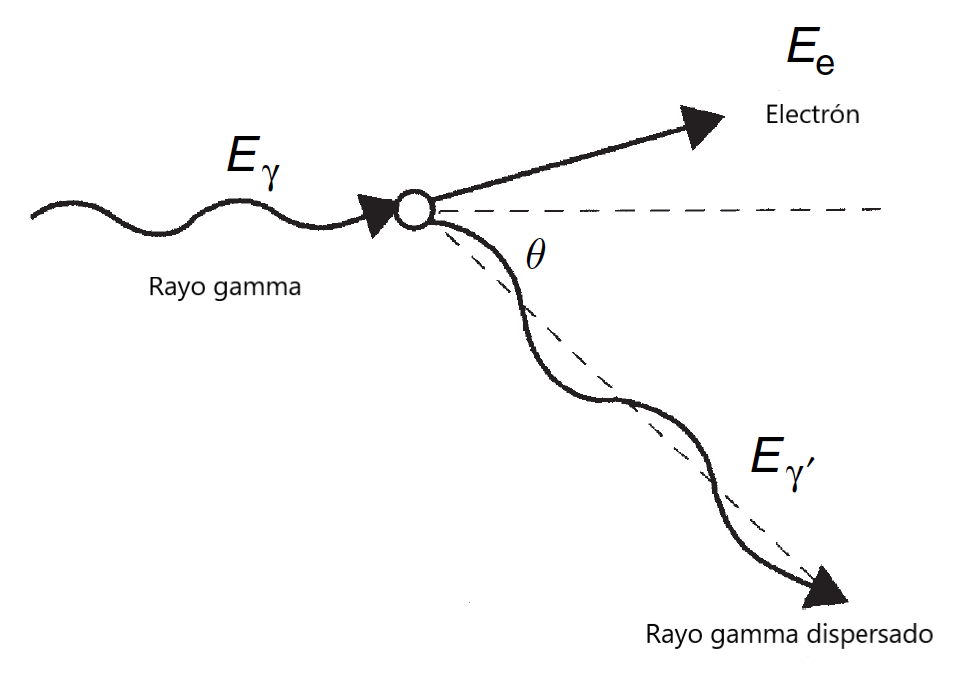
\includegraphics[width=0.48\textwidth]{Imagenes/Compton-2.png}
		\caption{Representación esquemática del efecto Compton, \cite{gilmore2008}.}\label{Fig-Compton}
		\end{figure}
		\subsubsection{Formación de pares}
A diferencia del efecto fotoeléctrico y Compton, la producción de pares es el resultado de la interacción del rayo gamma con el átomo en su conjunto. El proceso ocurre dentro del campo de Coulomb del núcleo y produce la conversión de un rayo gamma en un par electrón - positrón. Para que este proceso sea energéticamente posible, la energía del rayo gamma debe ser superior a la suma de la energía en reposo del electrón y positrón $E > 1.022$ MeV.
\vspace{0.5cm} \\
El positrón creado encuentra otro electrón y se aniquila emitiendo dos rayos gamma diametralmente opuestos de 511 keV cada uno. Para $E \gg m_e\,c^2$, la sección eficaz de la producción de pares $\sigma_{\text{pares}}$ se puede escribir como \cite{grupen2008particle}
\begin{equation}
\sigma_{\text{pares}} = \dfrac{7}{9}\,\dfrac{N_A}{A}\,\dfrac{1}{X_0}, \hspace{1cm}\text{con}\hspace{1cm} X_0 \propto\left[Z^2\,\log\left(\dfrac{183}{Z^{1/3}}\right) \right]^{-1}, 
\end{equation}
donde $N_A$ es el número de Avogadro y $A$ el número de nucleones.
\\ \\ 
La Figura \ref{Fig-Secciones} muestra la sección eficaz total por átomo en función de la energía para fotones sobre germanio ($Z=32$) y las contribuciones parciales de cada proceso de acuerdo al intervalo energético \cite{NistGE}. Para una energía de 46.54 keV (\PbCero) el proceso dominante es el efecto fotoeléctrico, sin embargo, para una energía de 351.93 (\PbCuatro) el efecto Compton es el proceso dominante. 
\begin{figure}[h]
\centering
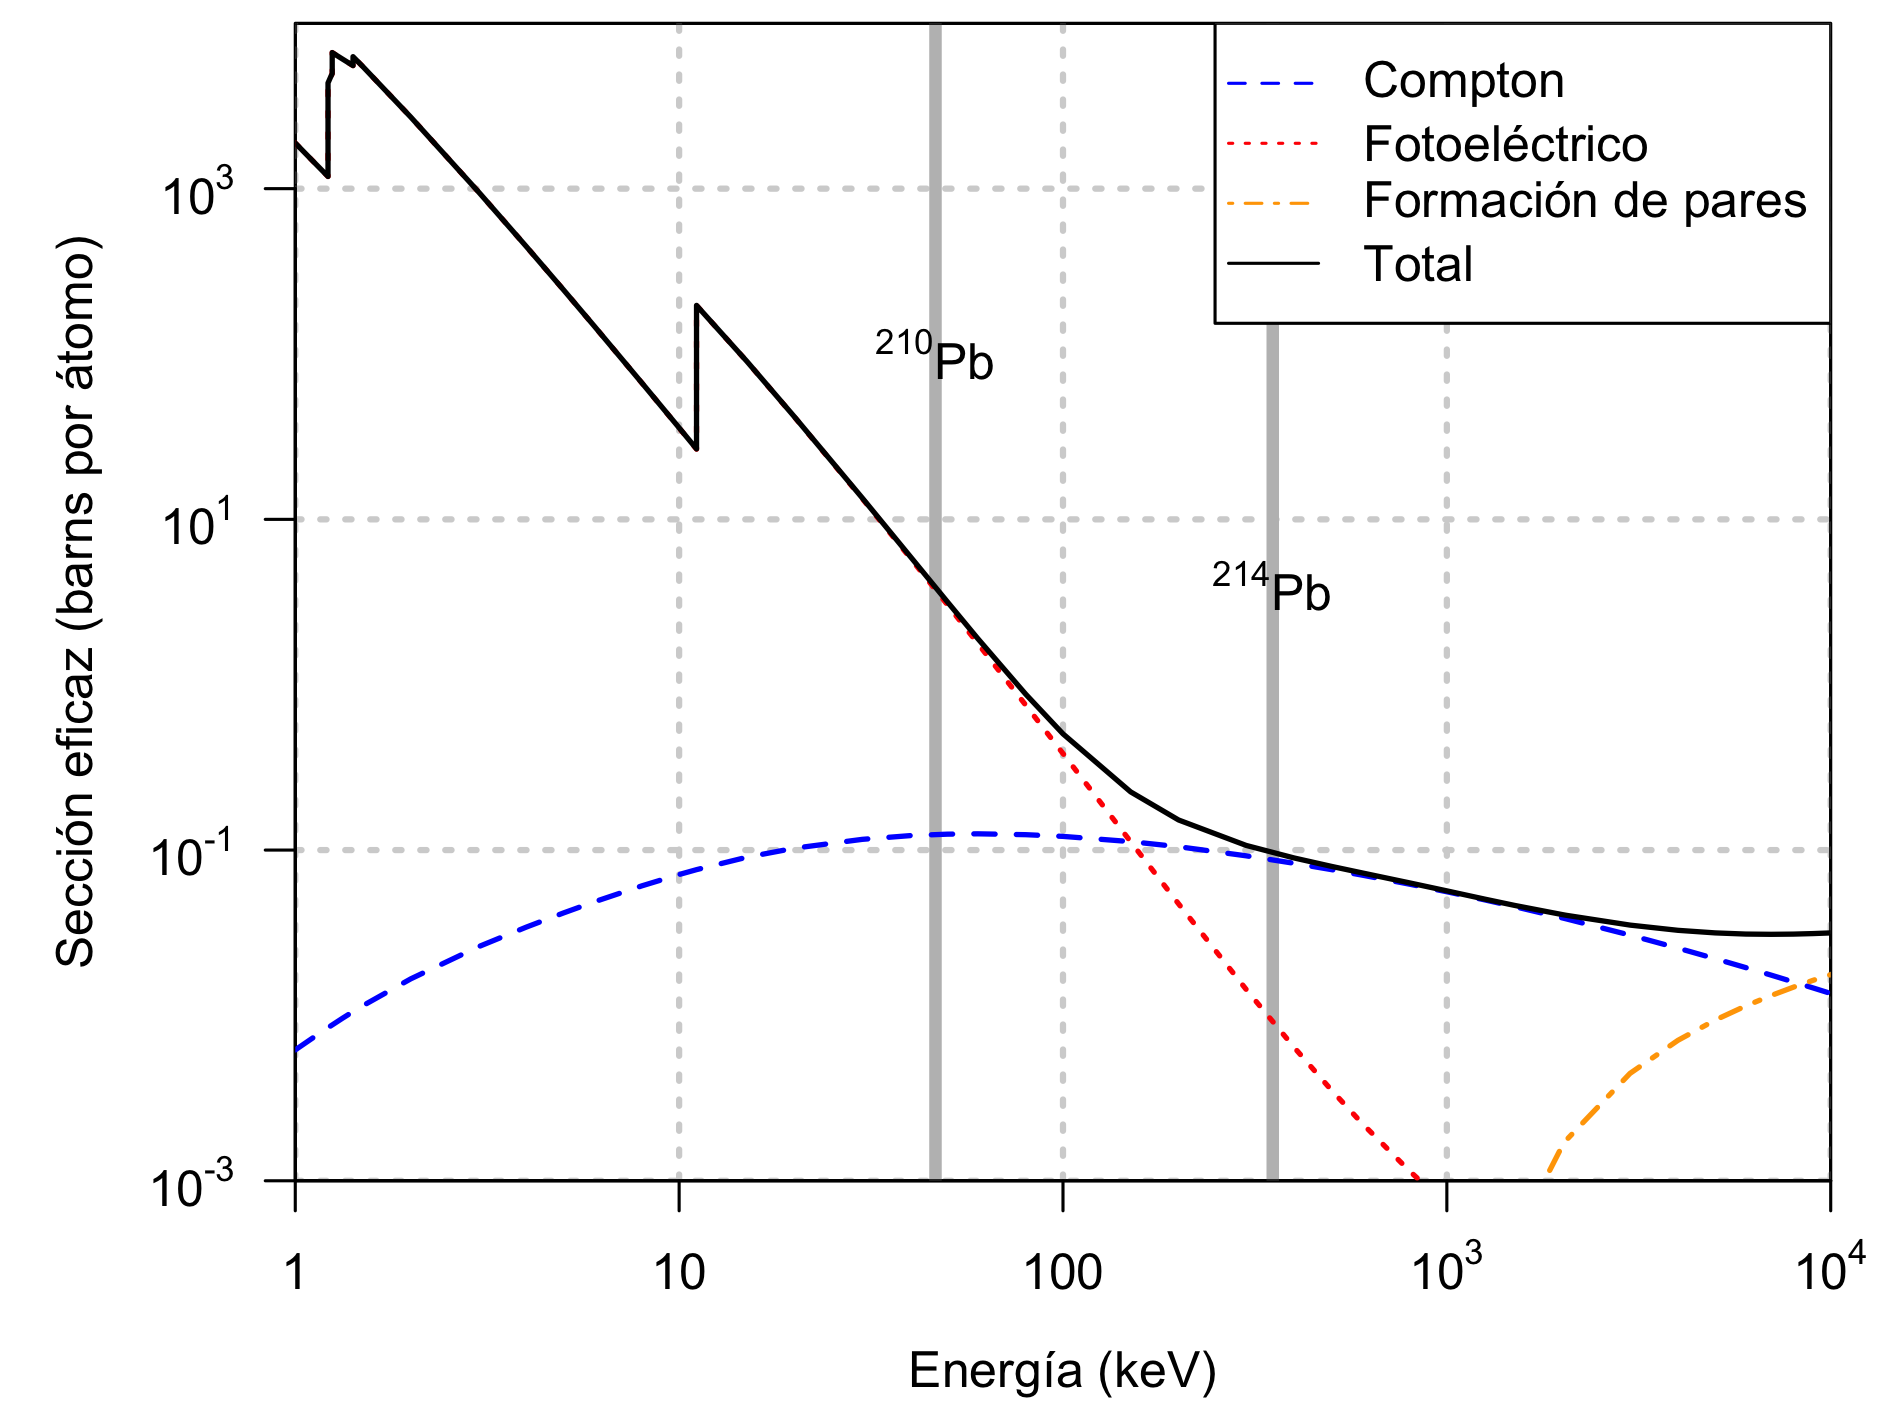
\includegraphics[width=0.7\textwidth]{Imagenes/CrossSectionGe.png}
\caption{Sección eficaz total de fotones sobre germanio $(Z=32)$. Se observan las contribuciones parciales de los procesos: fotoeléctrico, Compton y formación de pares.}\label{Fig-Secciones}
\end{figure}
		\subsubsection{Coeficiente másico de atenuación}
La interacción de la radiación con la materia se cuantifica de forma global a través del coeficiente másico de atenuación  $\dfrac{\mu}{\rho}$. Cuando un haz monoenergético y colimado de radiación gamma con intensidad inicial $I_0$ incide sobre un material de densidad $\rho$, su intensidad $I$ decrece siguiendo la ley de atenuación exponencial \cite{CUTSHALL1983309, NIST}
\begin{equation}\label{Eq-Atenuacion}
\dfrac{I}{I_0} = \exp\left[-\dfrac{\mu}{\rho}\,\rho\,x\right].
\end{equation}
La anterior ecuación es una aproximación porque asume que los rayos gamma perfectamente colimados atraviesan la muestra sin desviarse, si bien los fotones pueden emerger en ángulos diversos \cite{IURIAN2018151}. Los valores de $\dfrac{\mu}{\rho}$ para muchos materiales se encuentran ya reportados en \cite{NIST}.
\\
\\
La sección eficaz total $\sigma_\text{total}$, que es la suma de las secciones eficaces de los procesos considerados para determinada energía $E$, $\sigma_\text{total} = \sigma_\text{foto} + \sigma_\text{Comp} + \sigma_\text{pares} + ...$, se relaciona con el coeficiente másico de atenuación mediante \cite{NIST}
\begin{equation}\label{Eq-Mu}
\dfrac{\mu}{\rho} = \dfrac{\sigma_\text{total}}{u\,A},
\end{equation}
donde $\rho$ es la densidad del material, $u$ es la unidad de masa atómica y $A$ el número de nucleones. Por lo tanto, $\dfrac{\mu}{\rho}$ es un parámetro que depende de la energía del rayo gamma incidente y del material.
	\subsection{Detectores de Ge hiper-puro}\label{SubSec-DetecGe}
Los detectores de Ge hiper-puro son semiconductores, que presentan un comportamiento intermedio entre los materiales conductores y los materiales aislantes. La diferencia de energía entre la banda de valencia y la banda de conducción (gap - banda prohibida de energía) es de 0.67 eV, lo que implica que los electrones pueden ser excitados térmica u ópticamente. 
\\ \\
Los detectores semiconductores (como Si, Ge y GeAs) pueden ser entendidos  como cámaras de ionización de estado sólido. Debido a su alta densidad en comparación con los gases, los volúmenes de los detectores pueden ser muy inferiores. Estos se polarizan con dos electrodos que generan un campo eléctrico encargado de recoger los pares electrón-hueco producidos en el material. Debido a que el gap es pequeño, la cantidad de pares electrón-hueco producidos por unidad de energía depositada es alta, por lo que su resolución energética es muy buena. Sus principales aplicaciones son la espectrometría de rayos gamma y de partículas cargadas con alta resolución energética.
\\ \\
Los detectores pueden ser intrínsecos o dopados. Los detectores dopados pueden ser de tipo n, tipo p, compensados o altamente dopados. El tipo de detector en los detectores dopados depende de la valencia del material agregado. La unión de un semiconductor tipo n y tipo p crea una región de agotamiento, o \textit{depletion region}, importante para la detección de la radiación. El campo eléctrico que se crea en la región de desequilibrio causa que cualquier electrón o hueco creado en esta zona tienda hacia la zona de tipo n o de tipo p, respectivamente \cite{knoll2010radiation}. 
\\\\
Los detectores semiconductores intrínsecos, no dopados, son materiales de alta pureza (Tabla \ref{Table-PropiedadesSiGEe}). Algunas características de los detectores semiconductores son:
\begin{itemize}
\item Densidad elevada en comparación con detectores gaseosos. Esto implica una mayor pérdida de energía en distancias cortas y efectos difusivos más cortos, generando resoluciones espaciales de hasta 10 $\mu$m.
\item Baja energía de ionización (pocos eV para crear un par electrón – hueco) en comparación con detectores gaseosos (20 - 40 eV para crear un par de iones) o centelladores (400 - 1000 eV para crear un fotón).
\item Los detectores de Ge son ampliamente utilizados en física nuclear y necesitan refrigeración debido a su banda de energía prohibida tan pequeña. Los detectores de Si pueden operar a temperatura ambiente y son materiales estándar para detectores de vórtices y trayectorias de partículas elementales en física de altas energías.
\item Su precio es elevado debido al volumen y pureza del material, electrónica asociada y sistema de refrigeración.
\end{itemize}
\begin{table}[h]
 \centering
 \caption{Propiedades de los detectores semiconductores intrínsecos Si y Ge \cite{bertolini1968semiconductor}.}\label{Table-PropiedadesSiGEe}
 \begin{tabular}{|c|c|c|c|}\hline
\rowcolor{Blue2} Propiedad & unidad & Si & Ge \\ \hline
\rowcolor{Blue1} Número atómico & & 14 & 32 \\
\rowcolor{Blue1} Peso atómico & u & 28.09 & 72.60 \\
\rowcolor{Blue1} Densidad a 300 K & g cm$^{-3}$ & 2.33 & 5.32 \\
\rowcolor{Blue1} Banda prohibida a 300 K & eV & 1.115 & 0.665 \\
\rowcolor{Blue1} Energía por cada par electrón - hueco & eV & 3.76 & 2.96 \\ \hline
 \end{tabular}
\end{table}
			\subsubsection{Detectores de Ge en configuración tipo pozo}\label{Sec-GePozo}
Los detectores de Ge en configuración tipo pozo (Figura \ref{Fig-WellDetectorORTEC}) son detectores coaxiales con un contacto negativo en una apertura circular que permite introducir muestras pequeñas en ella. Este tipo de detector proporciona un ángulo sólido próximo a $4\pi$ y, en un intervalo de energías entre 50 keV a 200 keV, una eficiencia absoluta cercana al 90 \%, mientras que la eficiencia absoluta de los detectores de Ge cilíndricos comunes es muy inferior al 50 \% \cite{gilmore2008}.
\vspace{0.5cm}\\
La eficiencia absoluta es función de la energía y depende de la configuración geométrica: dimensiones del detector, del pozo y naturaleza del material protector del mismo (usualmente una capa de Al). La eficiencia adquiere su valor máximo en la parte inferior del pozo. La  capacitancia  de un detector de Ge en configuración tipo  pozo  es  mayor que la de un detector equivalente coaxial de Ge, causando una peor resolución  \cite{gilmore2008}.
\begin{figure}[h]
\centering
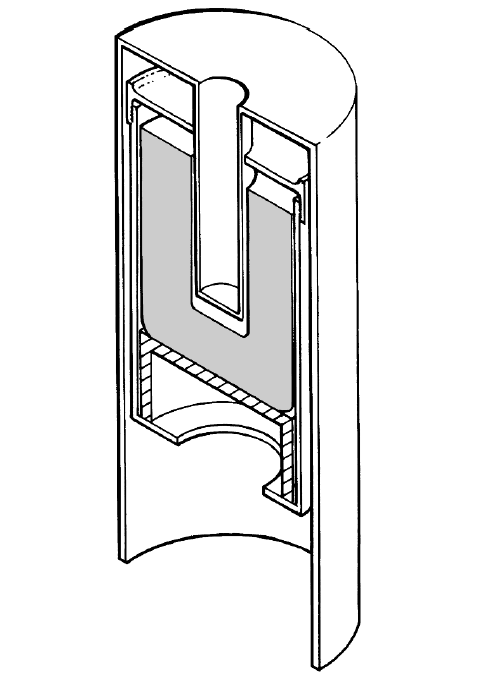
\includegraphics[width=0.25\textwidth]{Imagenes/WellDetectorSimply.png}
\caption{Vista isométrica simplificada de un detector de Ge en configuración de pozo \cite{WellDetectorORTEC}.}\label{Fig-WellDetectorORTEC}
\end{figure}
	\subsection{Eficiencia}\label{SubSec-Eficiencia}
La eficiencia absoluta $\epsilon$ para un sistema detector - fuente es la fracción entre el número de eventos emitidos y el número de eventos registrados, 
\begin{equation}
\epsilon = \dfrac{\text{Números de eventos registrados}}{\text{Número de eventos emitidos por la fuente}}.
\end{equation}
La eficiencia absoluta depende de i) la energía de la radiación emitida $E$, ii) la configuración geométrica detector – fuente, iii) la probabilidad de interacción de la radiación con el material –detector (eficiencia intrínseca), y iv)  la autoabsorción de la radiación en la muestra, entre otros factores. La eficiencia absoluta se puede escribir como \cite{PALACIOS200877}:
\begin{equation}
\epsilon(E) = \epsilon_{\text{intríseca}}(E)\cdot \epsilon(\Omega)\cdot\text{TCSC}\cdot \eta(E), 
\end{equation}
en donde 
\begin{itemize}
\item $\epsilon_{\text{intríseca}}(E)$ es la eficiencia intrínseca del detector a una energía determinada $E$. Se trata del número de eventos detectados en comparación con el número de eventos que impactan al detector. Es un parámetro básico y es independiente de la geometría fuente – detector,
\item $\epsilon(\Omega)$ es el factor geométrico. Esto se relaciona con la idea de un ángulo sólido entre la fuente y el detector,
\item TCSC (True Coincidence Summing Correction) es la corrección necesaria para corregir la detección simultánea de más de un rayo gamma o X. Este fenómeno es común en el caso de radionúclidos emisores gamma en cascada durante la desexcitación nuclear \cite{gilmore2008},
\item $\eta(E)$ es el factor de autoabsorción.
\end{itemize}
La actividad total $A$ (número de desintegraciones por unidad de tiempo) de un radionúclido en una muestra se determina mediante la ecuación: \cite{MONTALVANOLIVARES201734}
\begin{equation}\label{Eq-Actividad}
A = \dfrac{N(E) - B(E)}{\epsilon(E)\,f(E)\,t},
\end{equation}
en donde $N(E)$ es el número de cuentas netas para el fotopico $E$, $B(E)$ en el número de cuentas netas del fondo del detector para el mismo fotopico,  $\epsilon(E)$ es la eficiencia absoluta del sistema para la energía $E$, $f(E)$ es la probabilidad de emisión y $t$ es el tiempo de medición efectivo \cite{BELGIN201536}. La eficiencia absoluta puede ser determinada mediante calibración utilizando un patrón de geometría, composición y densidad similar a la muestra medida. Sin embargo, esto requiere la calibración directa de múltiples geometrías, densidades y composiciones en cada laboratorio, lo que es muy costoso y prácticamente imposible en la práctica.
\\ \\
Si bien una opción teóricamente posible es el cálculo de la eficiencia a través de simulación Monte Carlo de todos los procesos que ocurren desde la emisión del rayo gamma hasta su detección, una alternativa es la corrección de la eficiencia a través de funciones de transferencia \cite{VIDMAR2005603, MORERAGOMEZ201559}.
		\subsubsection{Factor de autoabsorción}\label{SubSecc-CoeffAtten}
La autoabsorción ocurre cuando parte de la radiación gamma emitida en una muestra extensa pierde parcial o totalmente su energía en la muestra misma y se cuantifica con el factor de autoabsorción $\eta(E)$. Este efecto es particularmente importante para rayos gamma de baja energía (como en el caso del \PbCero) y por lo tanto, afecta seriamente la exactitud de la medida de la actividad \cite{PILLEYRE2006323}.
\\
\\
El factor de autoabsorción depende de la composición, densidad y geometría de la muestra \cite{CUTSHALL1983309} y sigue la misma forma funcional que la Ecuación \ref{Eq-Atenuacion}. Para energías superiores a 80 keV, las diferencias en las composiciones químicas y densidades de muestras ambientales no afectan significativamente a $\dfrac{\mu}{\rho}$, pero sí afectan significativamente para energías inferiores \cite{VARGAS2002893}.
\\
\\
El factor de autoabsorción para materiales con diferentes composiciones puede calcularse mediante simulación Monte Carlo a través de la ecuación \cite{BELGIN201536, CUTSHALL1983309, APPLEBY1992228, APPLEBY2004423, PILLEYRE2006323, SAIDOU2007515}
\begin{equation}
\eta(E) = \exp\left(-\sum_i  \left( \dfrac{\mu}{\rho}\right)_i\,\rho_i\,x_i\right),
\end{equation}
donde el índice $i$ indica a los elementos que constituyen la muestra, $\left(\dfrac{\mu}{\rho}\right)_i$, $\rho_i $ y $x_i$ son el coeficiente másico de atenuación, densidad y concentración absoluta de cada elemento. 
		\subsubsection{ANGLE}\label{SubSec-ANGLE}
ANGLE es un software comercial que permite el cálculo de eficiencias mediante funciones de transferencia. La función de transferencia se define como el cociente de dos eficiencias y, por lo tanto, permite obtener la eficiencia $\epsilon$ partiendo de una eficiencia de referencia $\epsilon_\text{referencia}$. Una de las ventajas de esta estrategia es que las correcciones introducidas por la función de transferencia deberían ser pequeñas y, por lo tanto, sujetas a errores pequeños. 
\\
\\
La eficiencia se determina mediante ANGLE a través de un método semi-empírico que involucra i) la calibración experimental del detector para el cálculo de la eficiencia de referencia y, ii) una simulación mediante Monte Carlo que genera un \textit{ángulo sólido efectivo} de acuerdo a cierta composición y geometría. El ángulo sólido efectivo $\overline{\Omega}$ (Figura \ref{Fig-EffSolidAngle}) se define como \cite{JOVANOVIC2010385}
\begin{equation}\label{Eq-EffSolidAngle}
\overline{\Omega} = \int_{V_S, S_D}\, d\overline{\Omega} = \int_{V_S, S_D}\,\displaystyle F_{\text{aten.}}\,F_{\text{ef.}} \dfrac{\overrightarrow{TP}\cdot\hat{n}}{|\overrightarrow{TP}|^3}\,d\sigma,
\end{equation}
donde
\begin{itemize}
\item $V_S$: volumen de la muestra.
\item $S_D$: área del detector expuesta a la muestra.
\item $T$ y $P$ son puntos que varían sobre el volumen de la muestra y la superficie del detector, respectivamente. $\overrightarrow{TP}$ es la distancia entre estos dos puntos.
\item $d\sigma$: Elemento infinitesimal de área en $S_D$.
\item $\hat{n}$: vector unitario normal al diferencial de área $d\sigma$.
\item $F_{\text{aten.}}$: factor que toma en cuenta la atenuación del rayo gamma en dirección $\overrightarrow{TP}$.
\item $F_{\text{ef.}}$: probabilidad de interacción entre fotón y detector. 
\end{itemize}
La eficiencia $\epsilon$ para la energía de fotopico se calcula mediante la función de transferencia
\begin{equation}\label{Eq-Epsilon}
\epsilon = \dfrac{\overline{\Omega}}{\overline{\Omega}_\text{referencia}}\,\epsilon_\text{referencia}.
\end{equation}
La anterior ecuación asume que la eficiencia es una función intrínseca del detector y depende únicamente de la energía del rayo gamma.
\begin{figure}[h]
\centering
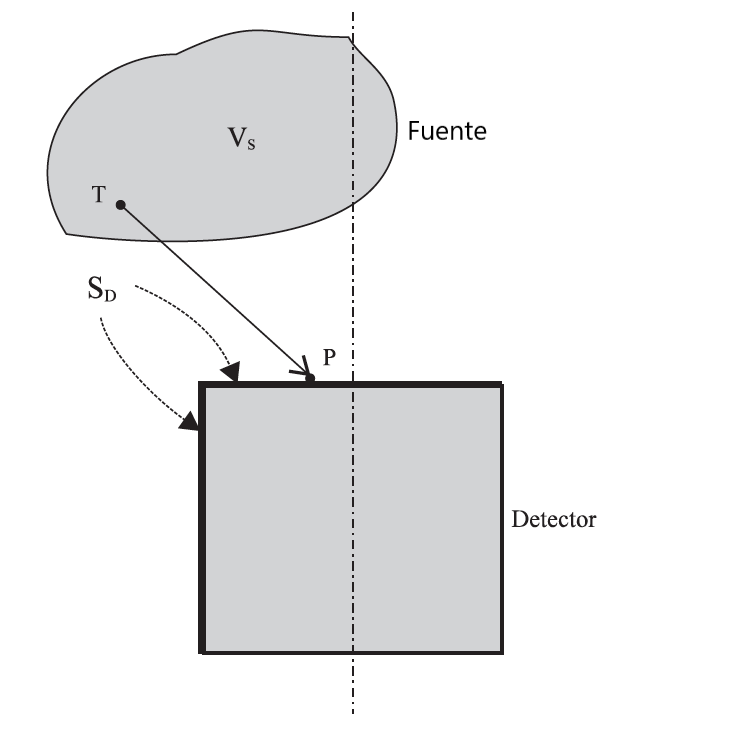
\includegraphics[width=0.45\textwidth]{Imagenes/EffectiveSolidAngle-2.png}
\caption{Variables involucradas en el cálculo del ángulo sólido efectivo, Ec. (\ref{Eq-EffSolidAngle}), para encontrar eficiencias a través del software ANGLE mediante la Ecuación \ref{Eq-Epsilon}.}\label{Fig-EffSolidAngle}
\end{figure}
\section{Análisis elemental}\label{Secc-AnalisisElemental}
El análisis de composición elemental de las muestras de núcleos sedimentarios se realizó en el Laboratorio de Geoquímica Isotópica y Geocronología (LGIG) de la UNAM mediante las técnicas de espectrometría de fluorescencia de rayos X (XRF, Sección \ref{SubSec-XRF-Intro}) y análisis elemental (Sección \ref{SubSec-CN-Intro}). XRF permitió analizar 48 elementos desde Na hasta U, en tanto que, las concentraciones de C y N se determinaron por analizador elemental.
	\subsection{Espectrometría de fluorescencia de rayos X}\label{SubSec-XRF-Intro}
XRF es una técnica analítica no destructiva que permite identificar y cuantificar la concentración de elementos químicos en una muestra. La técnica consiste en hacer incidir radiación electromagnética (rayos X) sobre la muestra para provocar la emisión de electrones atómicos. El lugar del electrón eyectado es ocupado por otro electrón de mayor energía que, en su transición, pierde energía en forma de rayos X característicos, lo que permite identificar el elemento. La emisión de rayos X es prácticamente inmediata ( $\sim 10^{-15}$ s), por lo que la emisión se considera fluorescente.  
\\
\\
El espectro de energías XRF está compuesto principalmente por las transiciones que ocurren cuando el átomo pierde un electrón de las subcapas 1s o 2s. Dado que los rayos X emitidos son característicos de cada átomo, pueden ser utilizados para establecer la concentración de cada elemento \cite{verma2007atomic}. 
	\subsection{Análisis elemental de C-N}\label{SubSec-CN-Intro}
El análisis cuantitativo de carbono y nitrógeno se realiza mediante la oxidación, reducción y separación de gases de la muestra durante su combustión. Los principales procedimientos para la cuantificación de estos elementos son  \cite{smith2003soil, danovaro2009methods} (Figura \ref{Fig-CN-Esquema}):
\begin{enumerate}
\item Oxidación de la muestra en CO$_2$, vapor de agua, N$_2$, N$_x$O$_y$, SO$_z$ y otros gases mediante la combustión a alta temperatura ($\sim$ 1200 \grados C).
\item Transporte de gases generados con He. 
\item Reducción de óxidos de nitrógeno producidos en N$_2$, CO$_2$ y HO$_2$. 
\item Eliminación de gases no deseados (como óxidos de Si).
\item Separación de gases mediante cromatografía de gases (detector de conductividad térmica) o series de trampas para cada gas.
\item Detección de los gases, comparación con curvas de calibración y cuantificación de concentraciones.
\end{enumerate}
La variación entre los analizadores elementales de C y N radica en el sistema de detección de los gases y en el sistema de análisis.
\begin{figure}[h]
\centering
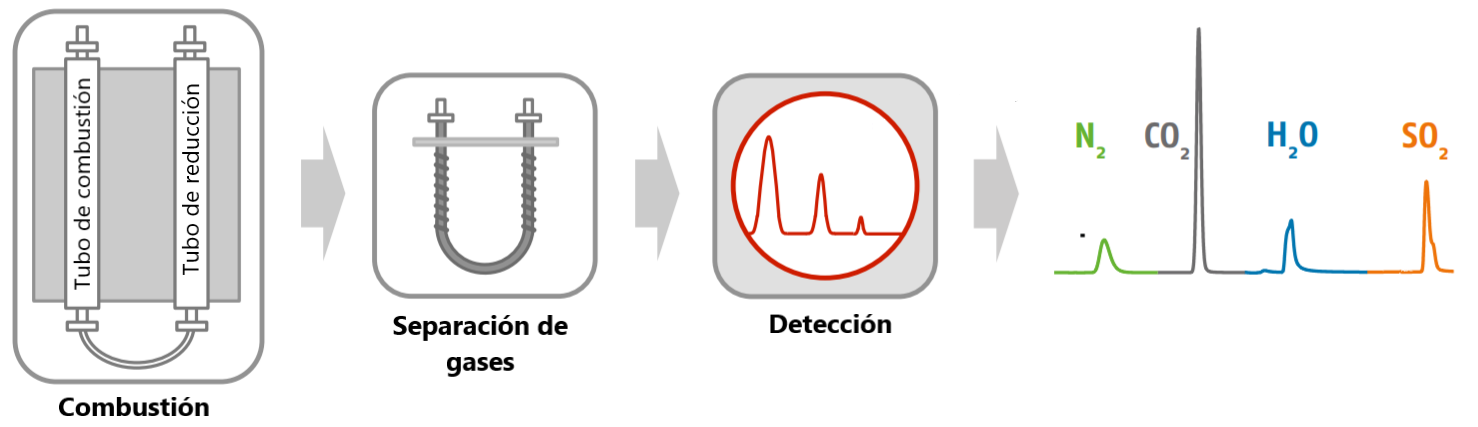
\includegraphics[width=0.9\textwidth]{Imagenes/C-N-Detection-2.png}
\caption{Procedimientos para el análisis elemental de carbono y nitrógeno: combustión, separación de gases y detección. Tomado de \textit{Flyer vario MICRO cube}, marca Elementar.}\label{Fig-CN-Esquema}
\end{figure}

\section{Simulaciones de Monte Carlo}\label{Secc-MonteCarlo}
Las simulaciones Monte Carlo son experimentos numéricos basados en variables de entrada con distribuciones de probabilidad establecidas y el modelo $z$ a explorar. En cada uno de los $N$ experimentos numéricos, los valores de las variables de entrada $x_i$, $1 \leq i \leq N$, se determina de acuerdo a sus distribuciones de probabilidades y los resultados son calculados mediante las relaciones del modelo $z = z(x_i)$ \cite{cruse1997reliability}. 
\\ \\ 
Las variables $x_i$ son variables aleatorias que adquieren un valor de un intervalo, finito o infinito, y siguen una función de densidad de probabilidad. Las funciones de densidad de probabilidad usuales son i) uniforme o rectangular, ii) exponencial, y iii) Gausiana. Típicamente, los resultados del modelo $z$ se expresan en términos de la media $\overline{z}$ y la varianza $\sigma^2(z)$, \cite{dunn2011exploring}
\begin{equation}
\overline{z} = \dfrac{1}{N}\sum_{i=1}^N z(x_i), \hspace{1cm} \sigma^2(z) = \dfrac{1}{N-1}\sum_{i=1}^N  (z(x_i) - \overline{z})^2.
\end{equation}
Según la ley de número grandes, si existen el valor medio y la desviación estándar, el valor promedio del modelo Monte Carlo tiende al valor real con el número de simulaciones $N\rightarrow \infty$, usualmente $N \sim 10^4$. 
\section{Hipótesis}\label{Sec-Hipotesis}
El fechado de núcleos sedimentarios con el radionúclido \PbCero\, requiere un conocimiento lo más aproximado posible de la actividad real de la muestra, la cual depende de la composición elemental de cada sección del núcleo sedimentario. El conocimiento de la composición elemental de cada sección permite conocer mejor la actividad real de cada muestra y obtener un fechado con \PbCero\, de mayor calidad. 
\section{Objetivos}\label{Sec-Objetivos}
El objetivo general de esta tesis es mejorar la cuantificación de los radionúclidos utilizados en el fechado de sedimentos recientes (\PbCero\, y \PbCuatro) a través de correcciones de densidad y autoabsorción específicas para cada muestra analizada. 
	\subsection{Objetivos específicos}\label{Sec-ObjEspec}
\begin{itemize}
\item Caracterizar los detectores de germanio hiper-puro tipo pozo utilizados en el LGIG: fondos, calibración de canal-energía y eficiencia-energía.
\item Seleccionar núcleos sedimentarios representativos de diversos sistemas acuáticos mexicanos. 
\item Determinar la composición elemental de algunas secciones de los núcleos  seleccionados y proponer su composición completa. 
\item Desarrollar códigos de programación para la lectura e integración de los datos provenientes de los equipos XRF y C-N, así como para ejecutar de manera sistemática el software ANGLE.
\item Estudiar los efectos de la densidad y composición elemental sobre la eficiencia de sistemas de espectrometría de rayos gammacon configuración de pozo para energías de 46.54 keV y 351.93 keV.
\item Estudiar el efecto de las correcciones realizadas en las actividades y el fechado de los núcleos seleccionados en relación a los resultados utilizando una composición de referencia (agua, composición química H$_2$O, densidad $\rho = 1$ g cm$^{-3}$). 
\end{itemize}
